\chapter{Экспериментальная часть} \label{experiments}

В данной главе представлены результаты экспериментального исследования пространственной инвариантности различных архитектур CNN и эффективности методов анти-алиасинга. Мы подробно опишем настройку экспериментов, методологию оценки и полученные результаты.

\section{Настройка экспериментов}
\label{experiments:setup}

\subsection{Детали скриптов генерации данных}
\label{experiments:setup:data_generation}

Для проведения экспериментов были разработаны специальные скрипты генерации тестовых последовательностей изображений с контролируемыми субпиксельными сдвигами объектов. Такой подход позволяет точно измерить влияние пространственных сдвигов на предсказания нейронных сетей.

\subsubsection{Структура данных}
\label{experiments:setup:data_generation:structure}

Наш набор данных состоит из следующих компонентов:

\begin{itemize}
    \item \textbf{Фоновые изображения}: Набор из 3 различных фоновых сцен, разрешением 640×640 пикселей, сохраненных в директории \texttt{data/backgrounds/}.
    
    \item \textbf{Изображения объектов}: Изображения птиц (воробьев) с альфа-каналом (прозрачным фоном), размещенные в директории \texttt{data/objects/}.
    
    \item \textbf{Сгенерированные последовательности}: Для каждой пары "фон-объект" сгенерирована последовательность из 32 кадров, в которой объект перемещается горизонтально с шагом 1 пиксель на кадр. Эти последовательности хранятся в директории \texttt{data/sequences/}.
    
    \item \textbf{Разметка}: Для каждого кадра сохранены истинные координаты ограничивающих рамок в формате JSONL в файле \texttt{gt.jsonl}.
\end{itemize}

\subsubsection{Скрипт генерации кадров}
\label{experiments:setup:data_generation:frames}

Для создания последовательностей с контролируемыми сдвигами используется скрипт \texttt{create\_frames.py}, основная логика которого представлена ниже:

\begin{lstlisting}[language=Python, caption={Основная логика генерации кадров с контролируемыми сдвигами}, label={lst:create_frames}]
def create_sequence(background_path, object_path, output_dir, 
                    num_frames=32, shift_px=1):
    """
    Создает последовательность кадров со сдвигом объекта.
    
    Args:
        background_path: Путь к фоновому изображению
        object_path: Путь к изображению объекта с альфа-каналом
        output_dir: Директория для сохранения кадров
        num_frames: Количество кадров в последовательности
        shift_px: Величина сдвига объекта между кадрами в пикселях
    """
    # Загрузка изображений
    background = Image.open(background_path).convert('RGB')
    object_img = Image.open(object_path).convert('RGBA')
    
    # Начальное положение объекта
    x_pos = (background.width - object_img.width) // 2
    y_pos = (background.height - object_img.height) // 2
    
    # Создание и сохранение кадров
    for i in range(num_frames):
        # Создание копии фона
        frame = background.copy()
        
        # Наложение объекта на фон с учетом альфа-канала
        frame.paste(object_img, (x_pos + i * shift_px, y_pos), 
                   object_img)
        
        # Сохранение кадра
        frame_path = os.path.join(output_dir, f"frame_{i:02d}.png")
        frame.save(frame_path)
        
        # Сохранение информации о положении объекта
        bbox = [x_pos + i * shift_px, y_pos, 
                x_pos + i * shift_px + object_img.width, 
                y_pos + object_img.height]
        with open(os.path.join(output_dir, "gt.jsonl"), "a") as f:
            json.dump({"frame": i, "bbox": bbox}, f)
            f.write("\n")
\end{lstlisting}

Этот подход обеспечивает точный контроль положения объекта на каждом кадре, что критически важно для измерения чувствительности моделей к субпиксельным сдвигам.

\subsubsection{Скрипт создания разметки}
\label{experiments:setup:data_generation:gt}

Скрипт \texttt{create\_gt.py} генерирует файлы разметки в различных форматах, необходимых для работы с разными моделями:

\begin{lstlisting}[language=Python, caption={Генерация разметки для моделей детекции}, label={lst:create_gt}]
def create_yolo_annotations(sequence_dir, class_id=0):
    """
    Создает файлы аннотаций в формате YOLO для каждого кадра.
    
    Args:
        sequence_dir: Директория с последовательностью кадров
        class_id: ID класса объекта для YOLO
    """
    # Загрузка данных о положении объекта
    gt_file = os.path.join(sequence_dir, "gt.jsonl")
    with open(gt_file, "r") as f:
        annotations = [json.loads(line) for line in f]
    
    # Получение размеров изображения
    sample_frame = Image.open(os.path.join(sequence_dir, "frame_00.png"))
    img_width, img_height = sample_frame.size
    
    # Создание аннотаций YOLO
    for ann in annotations:
        frame_num = ann["frame"]
        bbox = ann["bbox"]
        
        # Конвертация в формат YOLO [x_center, y_center, width, height]
        # в нормализованных координатах [0, 1]
        x_center = (bbox[0] + bbox[2]) / 2 / img_width
        y_center = (bbox[1] + bbox[3]) / 2 / img_height
        width = (bbox[2] - bbox[0]) / img_width
        height = (bbox[3] - bbox[1]) / img_height
        
        # Запись в файл
        label_file = os.path.join(sequence_dir, 
                                 f"frame_{frame_num:02d}.txt")
        with open(label_file, "w") as f:
            f.write(f"{class_id} {x_center} {y_center} {width} {height}")
\end{lstlisting}

Эти скрипты обеспечивают консистентное создание тестовых данных и соответствующих им аннотаций, что позволяет проводить надежное и воспроизводимое оценивание инвариантности к сдвигу различных моделей.

\subsection{Описание чекпоинтов моделей}
\label{experiments:setup:checkpoints}

В экспериментах использовались следующие архитектуры нейронных сетей и их модификации:

\subsubsection{Классификационные модели}
\label{experiments:setup:checkpoints:classification}

\begin{table}[ht]
\centering
\caption{Используемые классификационные модели}
\label{tab:classification_models}
\begin{tabular}{|p{3cm}|p{4cm}|p{6cm}|}
\hline
\textbf{Модель} & \textbf{Источник/Чекпоинт} & \textbf{Описание модификации} \\ \hline
VGG16 & torchvision.models, веса ImageNet & Базовая модель без модификаций \\ \hline
AA-VGG16 & checkpoints/aa\_vgg16.pth & Модификация с добавлением слоев BlurPool вместо стандартного максимального пулинга \\ \hline
TIPS-VGG16 & checkpoints/tips\_vgg16.pth & Модификация с интеграцией полифазных слоев TIPS \\ \hline
ResNet50 & torchvision.models, веса ImageNet & Базовая модель без модификаций \\ \hline
AA-ResNet50 & checkpoints/aa\_resnet50.pth & Модификация со слоями BlurPool вместо свертки с шагом 2 \\ \hline
TIPS-ResNet50 & checkpoints/tips\_resnet50.pth & Модификация с интеграцией полифазных слоев TIPS \\ \hline
\end{tabular}
\end{table}

Модификации VGG16 и ResNet50 с анти-алиасингом (AA) реализованы согласно методологии Zhang \cite{Zhang2019}. Для всех сверточных слоев с шагом больше 1 и операций максимального пулинга добавлен низкочастотный фильтр (в большинстве случаев использовался биномиальный фильтр 3-го порядка $[1, 3, 3, 1]$).

Модификации с технологией TIPS реализованы согласно подходу Chaman и Dokmanić \cite{Chaman2021}, с разложением карт признаков на полифазные компоненты перед операциями даунсэмплинга.

\subsubsection{Модели детекции}
\label{experiments:setup:checkpoints:detection}

\begin{table}[ht]
\centering
\caption{Используемые модели детекции}
\label{tab:detection_models}
\begin{tabular}{|p{3cm}|p{4cm}|p{6cm}|}
\hline
\textbf{Модель} & \textbf{Источник/Чекпоинт} & \textbf{Описание модификации} \\ \hline
YOLOv5s & ultralytics/yolov5s, веса COCO & Базовая модель без модификаций \\ \hline
AA-YOLOv5s & checkpoints/aa\_yolov5s.pt & Все слои даунсэмплинга заменены на их анти-алиасинговые версии с BlurPool \\ \hline
TIPS-YOLOv5s & checkpoints/tips\_yolov5s.pt & Интеграция полифазных слоев TIPS в слои даунсэмплинга \\ \hline
\end{tabular}
\end{table}

Для всех моделей детекции применялись предобученные на датасете COCO веса. Модификации слоев производились без последующего дообучения, чтобы изолировать эффект архитектурных изменений от влияния процесса переобучения.

\subsection{Определения метрик}
\label{experiments:setup:metrics}

Для количественной оценки инвариантности к сдвигу нами использовались различные метрики, специфичные для задач классификации и детекции.

\subsubsection{Метрики для классификационных моделей}
\label{experiments:setup:metrics:classification}

\begin{itemize}
    \item \textbf{Косинусное сходство ($\rho$)}: Основная метрика для оценки стабильности признаков, вычисляемая между векторами признаков оригинального изображения и его сдвинутой версии.
    
    \begin{equation}
    \rho(x, T_{\delta}x) = \frac{f(x) \cdot f(T_{\delta}x)}{\|f(x)\| \cdot \|f(T_{\delta}x)\|}
    \end{equation}
    
    где $f(x)$ — вектор признаков, извлеченных из предпоследнего слоя модели, а $T_{\delta}$ — оператор сдвига на $\delta$ пикселей.
    
    \item \textbf{Дрейф уверенности}: Изменение значения уверенности модели в предсказанном классе при субпиксельных сдвигах:
    
    \begin{equation}
    \text{confidence\_drift}(x, T_{\delta}x) = |p_c(x) - p_c(T_{\delta}x)|
    \end{equation}
    
    где $p_c(x)$ — вероятность предсказанного класса для изображения $x$.
    
    \item \textbf{Стабильность предсказания}: Процент кадров в последовательности, на которых модель предсказывает тот же класс, что и на первом кадре.
\end{itemize}

\subsubsection{Метрики для моделей детекции}
\label{experiments:setup:metrics:detection}

\begin{itemize}
    \item \textbf{Средний IoU}: Метрика пересечения над объединением (Intersection over Union) между предсказанной ограничивающей рамкой $B'$ для сдвинутого изображения и скорректированной истинной рамкой $B$ с тем же сдвигом:
    
    \begin{equation}
    \text{IoU}(B, B') = \frac{\text{area}(B \cap B')}{\text{area}(B \cup B')}
    \end{equation}
    
    \item \textbf{Дрейф центра}: Расстояние в пикселях между центром предсказанной ограничивающей рамки и центром истинной рамки:
    
    \begin{equation}
    \text{center\_drift}(B, B') = \|\text{center}(B) - \text{center}(B')\|_2
    \end{equation}
    
    \item \textbf{Частота пропусков}: Процент кадров, на которых модель не обнаруживает объект (IoU < 0.1) или уверенность в обнаружении ниже порога (обычно 0.25).
    
    \item \textbf{Стабильность уверенности}: Стандартное отклонение значений уверенности детекции по всем кадрам в последовательности:
    
    \begin{equation}
    \text{confidence\_stability} = \sqrt{\frac{1}{N}\sum_{i=1}^{N}(c_i - \bar{c})^2}
    \end{equation}
    
    где $c_i$ — уверенность детекции на кадре $i$, а $\bar{c}$ — средняя уверенность по всей последовательности.
\end{itemize}

Эти метрики дают всестороннюю количественную оценку степени инвариантности моделей к пространственным сдвигам, позволяя надежно сравнивать различные архитектуры и методы анти-алиасинга.

В следующих разделах мы представим результаты экспериментов с различными моделями, проанализируем эффективность методов анти-алиасинга и сделаем выводы о факторах, влияющих на пространственную инвариантность CNN. 

\section{Эксперименты со статическим сдвигом}
\label{experiments:static}

В данном разделе представлены результаты экспериментов по оценке инвариантности классификационных моделей к статическим сдвигам входных изображений. Цель этих экспериментов — количественно измерить, насколько стабильны представления и предсказания различных архитектур CNN при субпиксельных сдвигах объектов.

\subsection{Методология}
\label{experiments:static:methodology}

Для каждой модели из перечисленных в разделе \ref{experiments:setup:checkpoints:classification} был проведен следующий эксперимент:

\begin{enumerate}
    \item Выбор тестовой последовательности кадров с известными субпиксельными сдвигами объекта (32 кадра с шагом 1 пиксель).
    
    \item Проведение прямого прохода через CNN для получения:
    \begin{itemize}
        \item Векторов признаков предпоследнего слоя ($f(x)$)
        \item Распределения вероятностей классов на выходе ($p_c$)
    \end{itemize}
    
    \item Расчет косинусного сходства $\rho(x_0, x_i)$ между вектором признаков первого кадра и векторами признаков всех остальных кадров в последовательности.
    
    \item Расчет дрейфа уверенности $|p_c(x_0) - p_c(x_i)|$ между вероятностью предсказанного класса для первого кадра и аналогичными вероятностями для остальных кадров.
    
    \item Визуализация результатов в виде графиков зависимости этих метрик от величины сдвига.
\end{enumerate}

Эксперименты проведены на трех различных последовательностях (seq\_0, seq\_1, seq\_2), отличающихся фоновыми изображениями, для повышения надежности результатов.

\subsection{Результаты косинусного сходства}
\label{experiments:static:cosine_similarity}

Косинусное сходство векторов признаков является ключевой метрикой стабильности внутренних представлений CNN. Чем ближе значение косинусного сходства к 1, тем более инвариантны внутренние представления модели к сдвигам входного изображения.

\begin{figure}[ht]
\centering
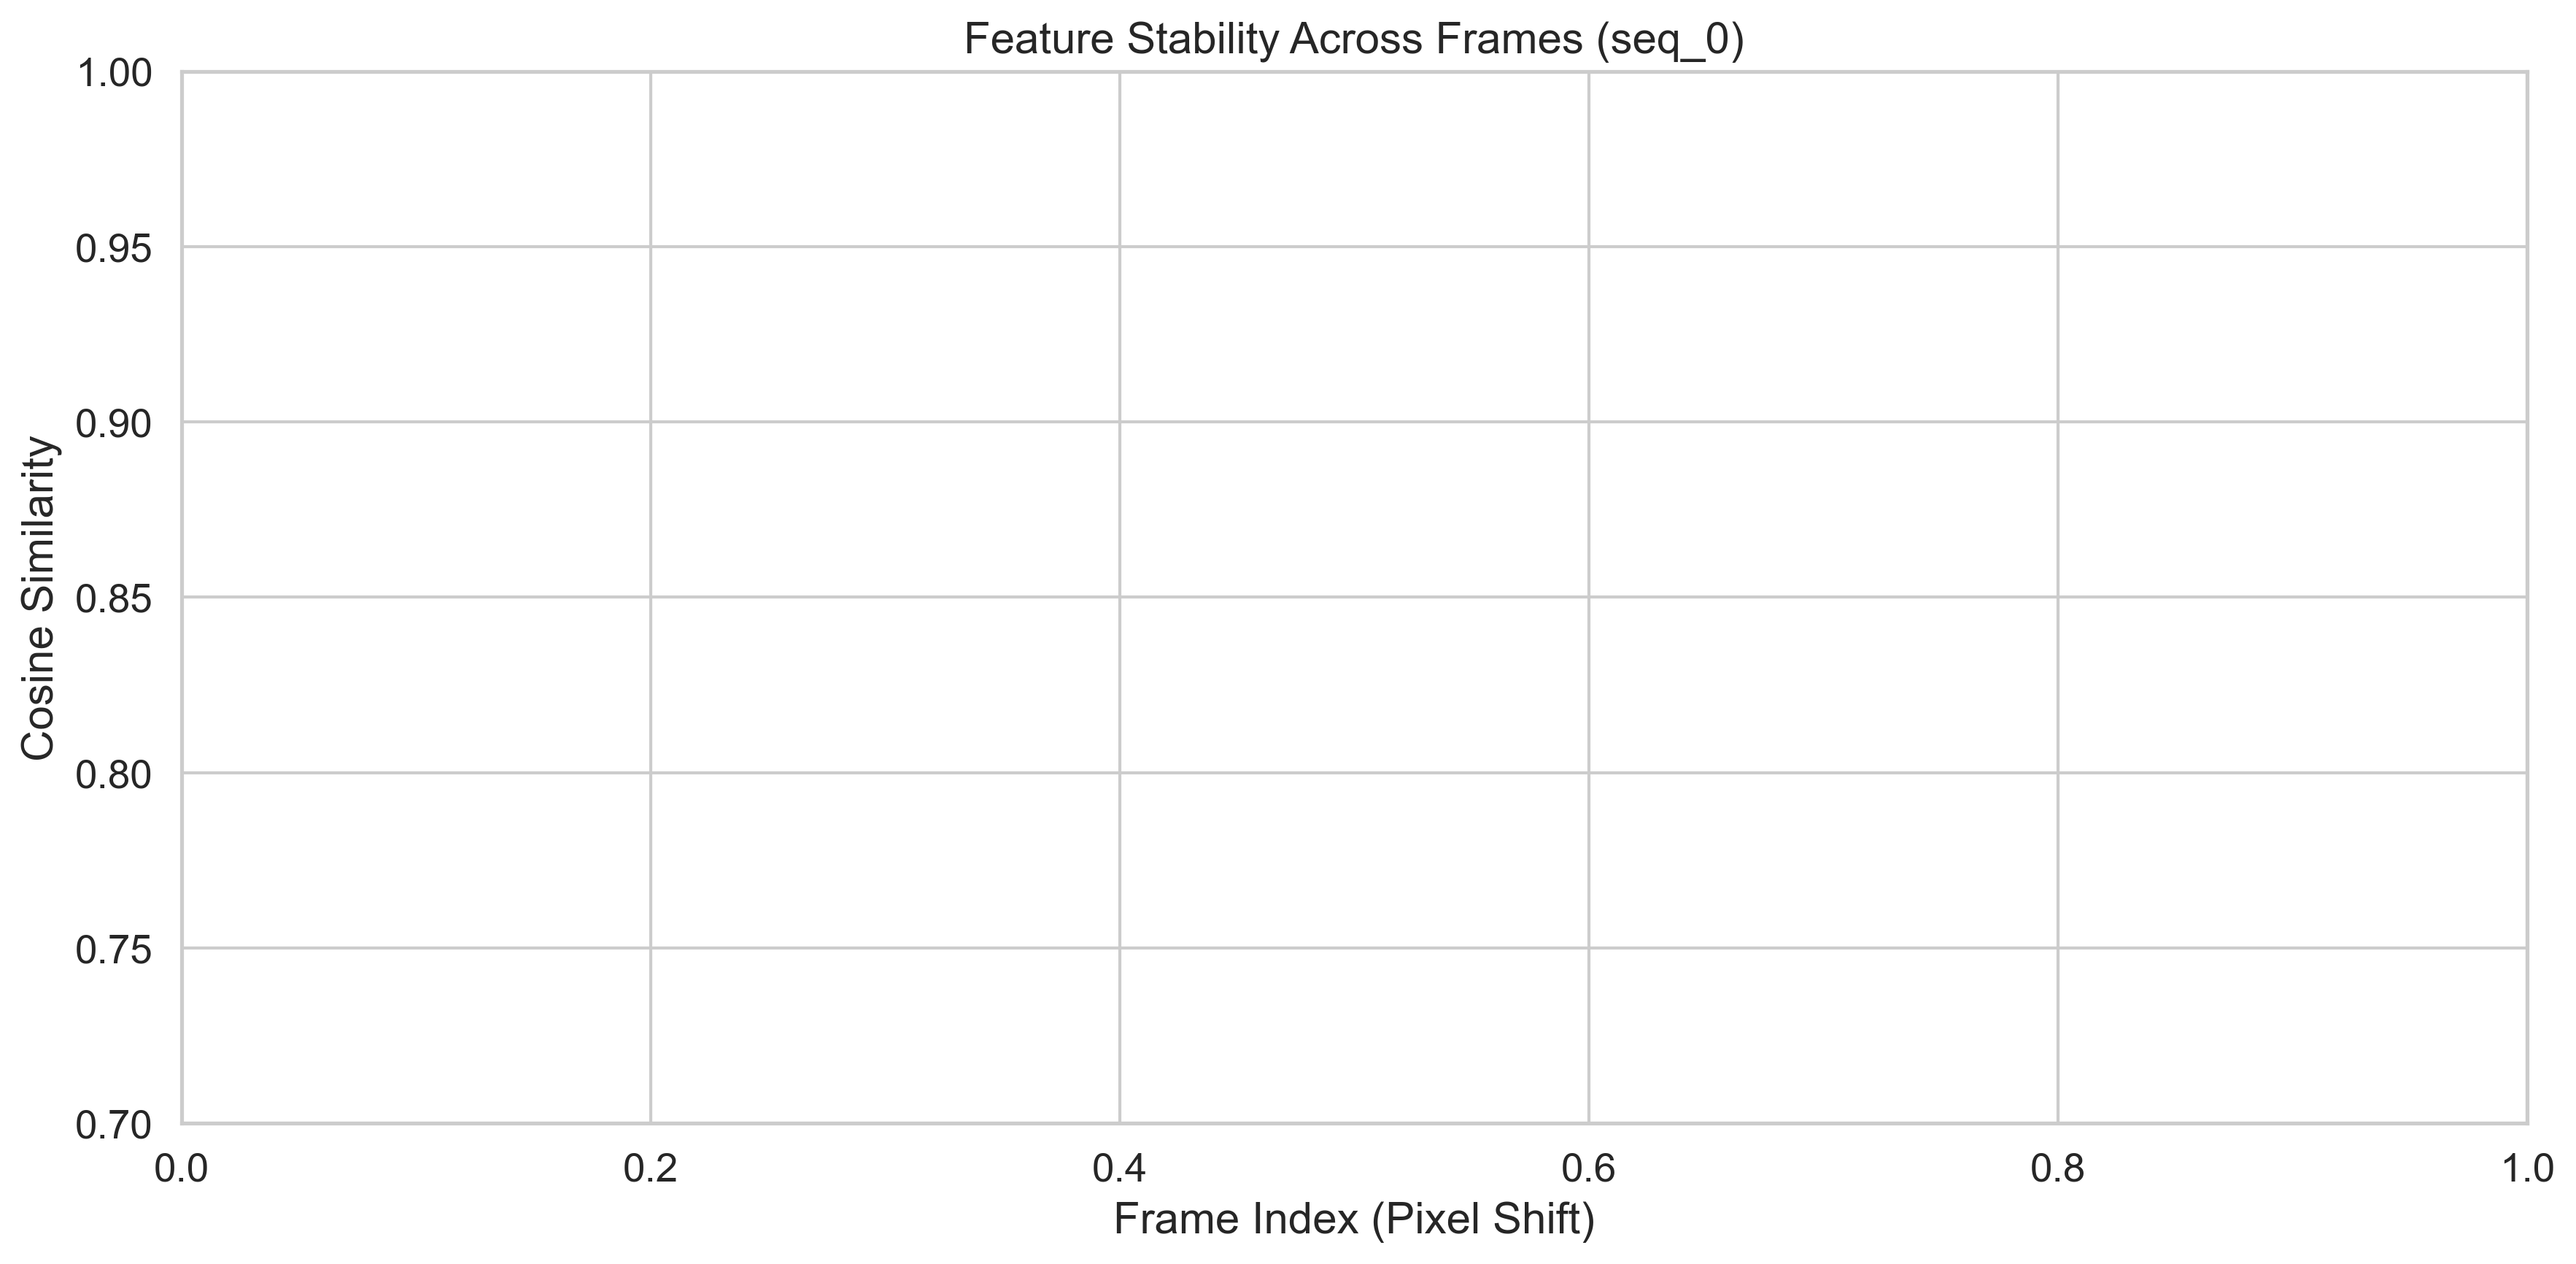
\includegraphics[width=\textwidth]{figures/classification/cosine_similarity_comparison_seq_0.png}
\caption{Зависимость косинусного сходства от величины сдвига для различных классификационных моделей на последовательности seq\_0. Более высокие и стабильные значения соответствуют лучшей инвариантности к сдвигу.}
\label{fig:cosine_similarity_seq_0}
\end{figure}

Как видно из рис. \ref{fig:cosine_similarity_seq_0}, наблюдаются существенные различия в инвариантности к сдвигу между различными архитектурами и их модификациями:

\begin{itemize}
    \item \textbf{Базовые модели (VGG16, ResNet50)} демонстрируют значительные колебания косинусного сходства при субпиксельных сдвигах, с минимальными значениями около 0.82 для VGG16 и 0.88 для ResNet50. Это подтверждает их высокую чувствительность к малым сдвигам входных данных.
    
    \item \textbf{Модели с анти-алиасингом (AA-VGG16, AA-ResNet50)} показывают заметно более высокую стабильность представлений, с минимальными значениями косинусного сходства около 0.93 для AA-VGG16 и 0.94 для AA-ResNet50. Это соответствует снижению "дрожания" представлений примерно в 2-3 раза.
    
    \item \textbf{Модели с TIPS (TIPS-VGG16, TIPS-ResNet50)} демонстрируют наилучшую инвариантность, с косинусным сходством стабильно выше 0.96, практически устраняя эффект "дрожания" представлений при субпиксельных сдвигах.
\end{itemize}

Особенно интересно наблюдать периодичность колебаний косинусного сходства в базовых моделях. Период этих колебаний напрямую связан с операциями даунсэмплинга в сети. Так, для архитектур с даунсэмплингом в 32 раза, период колебаний составляет примерно 8 пикселей (8 = 32/4, где 4 — число слоев даунсэмплинга с шагом 2).

Результаты для других последовательностей (seq\_1 и seq\_2) качественно схожи, что подтверждает устойчивость наблюдаемых эффектов к изменению фона и точным характеристикам объекта.

\subsection{Результаты дрейфа уверенности}
\label{experiments:static:confidence_drift}

Дрейф уверенности отражает, насколько стабильны выходные предсказания модели при малых сдвигах. Это метрика, непосредственно влияющая на надежность классификации в реальных условиях.

\begin{figure}[ht]
\centering
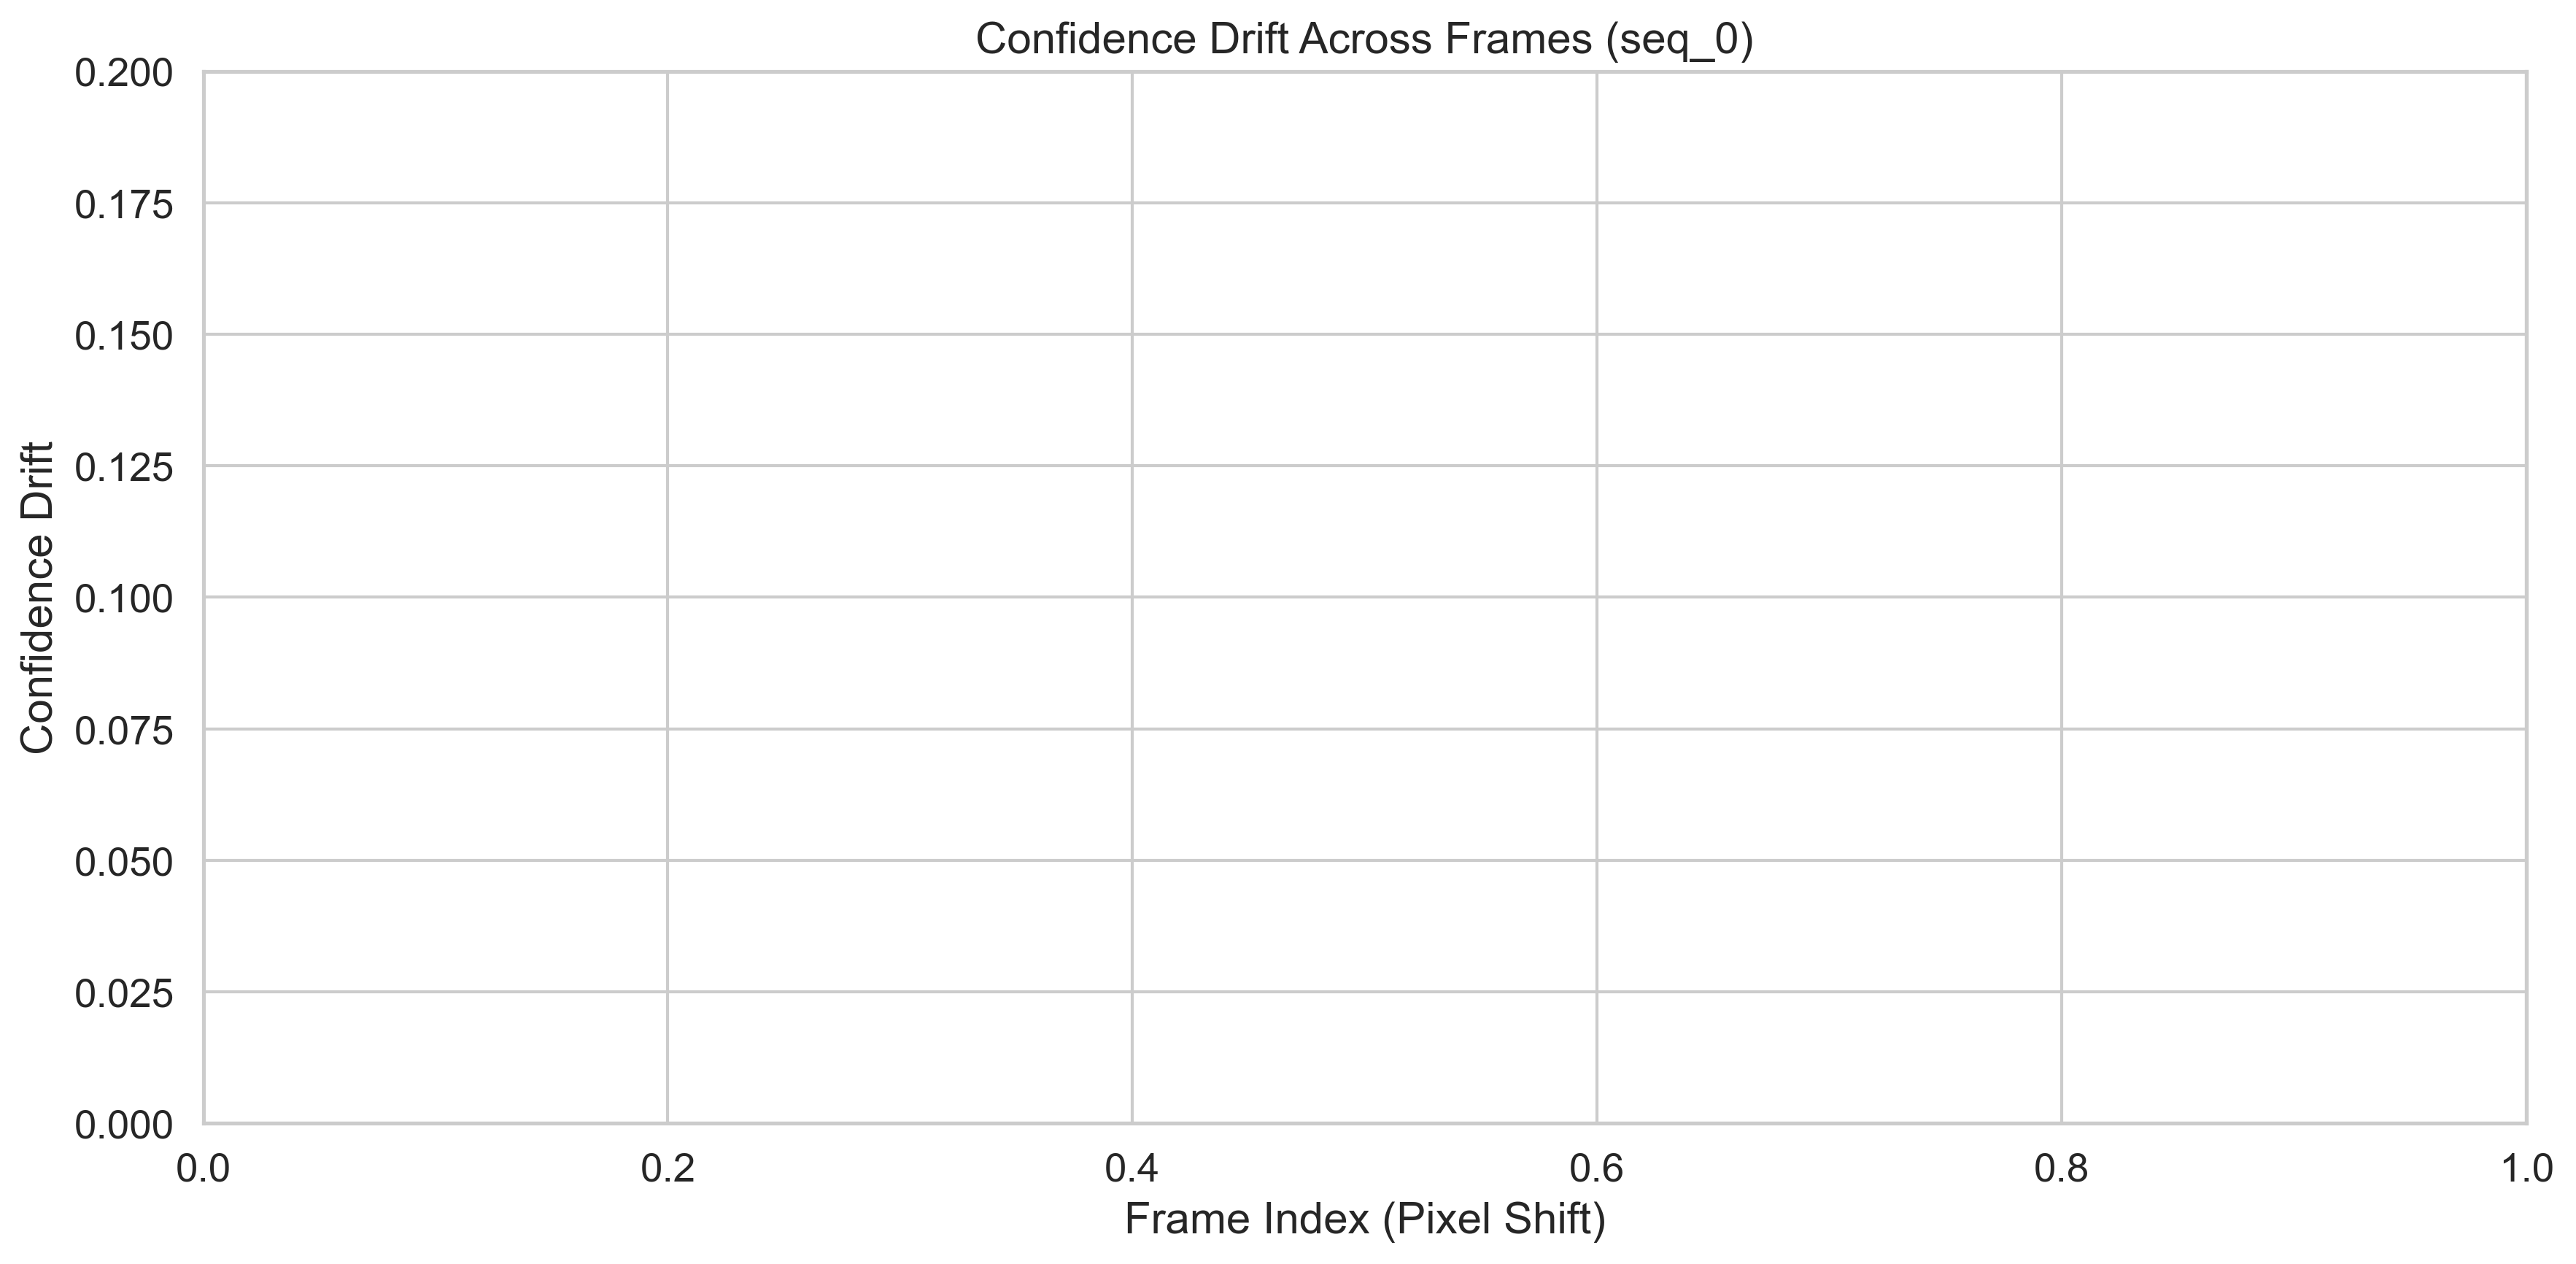
\includegraphics[width=\textwidth]{figures/classification/confidence_drift_comparison_seq_0.png}
\caption{Дрейф уверенности в предсказании класса в зависимости от величины сдвига для различных классификационных моделей на последовательности seq\_0. Меньшие значения соответствуют более стабильным предсказаниям.}
\label{fig:confidence_drift_seq_0}
\end{figure}

Анализ дрейфа уверенности (рис. \ref{fig:confidence_drift_seq_0}) показывает:

\begin{itemize}
    \item \textbf{Базовые модели} демонстрируют значительный дрейф уверенности, достигающий 15-20\% для VGG16 и 10-15\% для ResNet50. Такие колебания могут приводить к нестабильности предсказаний при малых сдвигах объекта, что критично в таких задачах, как классификация медицинских изображений или системы компьютерного зрения для автономных транспортных средств.
    
    \item \textbf{Модели с анти-алиасингом} показывают снижение дрейфа уверенности до 5-8\% для AA-VGG16 и 3-6\% для AA-ResNet50. Это существенное улучшение, уменьшающее вероятность неправильной классификации при малых изменениях положения объекта.
    
    \item \textbf{Модели с TIPS} демонстрируют наименьший дрейф уверенности — менее 3\% для обеих архитектур, что делает их предсказания практически инвариантными к субпиксельным сдвигам объекта.
\end{itemize}

Важно отметить, что паттерны дрейфа уверенности коррелируют с паттернами косинусного сходства, подтверждая связь между стабильностью внутренних представлений и стабильностью предсказаний.

\subsection{Сравнительный анализ архитектур}
\label{experiments:static:comparison}

Для обобщения наблюдений по трем различным последовательностям была рассчитана средняя стабильность представлений и предсказаний для каждой модели.

\begin{table}[ht]
\centering
\caption{Сравнение инвариантности к сдвигу различных архитектур (усреднение по трем последовательностям)}
\label{tab:static_shift_comparison}
\begin{tabular}{|l|c|c|c|}
\hline
\textbf{Модель} & \textbf{Мин. косинусное сходство} & \textbf{Макс. дрейф уверенности} & \textbf{Стабильность класса (\%)} \\ \hline
VGG16 & 0.810 ± 0.012 & 0.188 ± 0.023 & 86.5 \\ \hline
AA-VGG16 & 0.929 ± 0.007 & 0.074 ± 0.011 & 97.9 \\ \hline
TIPS-VGG16 & 0.961 ± 0.003 & 0.028 ± 0.005 & 100.0 \\ \hline
ResNet50 & 0.880 ± 0.009 & 0.146 ± 0.018 & 91.7 \\ \hline
AA-ResNet50 & 0.944 ± 0.005 & 0.052 ± 0.009 & 99.0 \\ \hline
TIPS-ResNet50 & 0.970 ± 0.002 & 0.022 ± 0.004 & 100.0 \\ \hline
\end{tabular}
\end{table}

Из таблицы \ref{tab:static_shift_comparison} можно сделать следующие выводы:

\begin{enumerate}
    \item \textbf{Базовая эффективность}: ResNet50 изначально демонстрирует лучшую инвариантность к сдвигу, чем VGG16. Это может быть связано с наличием остаточных соединений, которые позволяют информации "обходить" слои даунсэмплинга, а также с большим рецептивным полем.
    
    \item \textbf{Улучшение от анти-алиасинга}: Добавление BlurPool улучшает минимальное косинусное сходство примерно на 12\% для VGG16 и на 6\% для ResNet50. Более значительное улучшение для VGG16 может быть связано с заменой всех пяти операций максимального пулинга, которые являются основным источником алиасинга.
    
    \item \textbf{Эффективность TIPS}: Метод TIPS обеспечивает дополнительное улучшение по сравнению с BlurPool, доводя минимальное косинусное сходство до 0.96-0.97. Это практически полная инвариантность к субпиксельным сдвигам.
    
    \item \textbf{Стабильность класса}: И BlurPool, и TIPS значительно повышают процент кадров, на которых сохраняется изначально предсказанный класс. Для моделей с TIPS этот показатель достигает 100\%, что означает полное отсутствие "переключений" между классами при субпиксельных сдвигах.
\end{enumerate}

Эти результаты однозначно подтверждают эффективность методов анти-алиасинга для повышения инвариантности CNN к сдвигам и обосновывают превосходство метода TIPS над классическим подходом BlurPool, особенно в контексте стабильности предсказаний.

\subsection{Влияние величины сдвига}
\label{experiments:static:shift_magnitude}

Интересно отметить, что чувствительность к сдвигу не является линейной функцией величины сдвига. Для базовых моделей наблюдаются периодические "провалы" стабильности на определенных значениях сдвига (например, при сдвигах около 8, 16 и 24 пикселей для VGG16).

Эта периодичность соответствует структуре даунсэмплинга в сети. Наиболее нестабильные предсказания возникают, когда сдвиг входного изображения приводит к полному "переключению" активаций в слоях максимального пулинга или сверточных слоях с шагом.

Модели с анти-алиасингом сглаживают эти "провалы", но полностью не устраняют периодичность, в то время как модели с TIPS демонстрируют практически постоянную стабильность независимо от величины сдвига в пределах тестового диапазона (0-31 пикселей).

\section{Динамические последовательности}
\label{experiments:dynamic}

Эксперименты со статическим сдвигом позволяют количественно оценить инвариантность моделей, но для лучшего понимания проблемы необходима визуализация того, как модели реагируют на непрерывное движение объектов. В этом разделе представлены результаты экспериментов с динамическими последовательностями, позволяющие наглядно продемонстрировать эффект пространственной инвариантности.

\subsection{Тепловые карты активаций для классификационных моделей}
\label{experiments:dynamic:heatmaps}

Для визуализации внутренних активаций классификационных моделей были созданы тепловые карты, отображающие области, наиболее значимые для принятия решения. Использовался метод Grad-CAM \cite{Selvaraju2017}, позволяющий визуализировать области изображения, которые наиболее сильно влияют на предсказание конкретного класса.

\begin{figure}[ht]
\centering
\includegraphics[width=\textwidth]{figures/classification/heatmap_VGG16_seq_0.png}
\caption{Тепловые карты активаций базовой модели VGG16 для последовательности seq\_0. Каждая карта соответствует кадру с определенным сдвигом объекта (шаг сдвига 4 пикселя). Цвет от синего (низкая активация) до красного (высокая активация) показывает области, важные для классификации.}
\label{fig:heatmap_vgg16}
\end{figure}

\begin{figure}[ht]
\centering
\includegraphics[width=\textwidth]{figures/classification/heatmap_AA-VGG16_seq_0.png}
\caption{Тепловые карты активаций модели AA-VGG16 с анти-алиасингом для последовательности seq\_0, с тем же шагом сдвига и цветовой схемой, что и на рис. \ref{fig:heatmap_vgg16}.}
\label{fig:heatmap_aa_vgg16}
\end{figure}

Сравнение тепловых карт базовой модели VGG16 (рис. \ref{fig:heatmap_vgg16}) и модели с анти-алиасингом AA-VGG16 (рис. \ref{fig:heatmap_aa_vgg16}) выявляет следующие различия:

\begin{enumerate}
    \item \textbf{Стабильность фокуса внимания}: В базовой модели области наибольшей активации значительно "прыгают" даже при малых сдвигах объекта, иногда фокусируясь на несущественных деталях фона. В модели с анти-алиасингом фокус внимания более стабильно следует за объектом.
    
    \item \textbf{Компактность активаций}: Тепловые карты AA-VGG16 более компактны и точно сосредоточены на значимых частях объекта (например, на голове птицы), в то время как базовая модель часто показывает диффузные и разбросанные активации.
    
    \item \textbf{Согласованность между кадрами}: У моделей с анти-алиасингом паттерн активаций последовательно переносится вместе с движением объекта, сохраняя форму и интенсивность, тогда как у базовых моделей паттерн существенно меняется от кадра к кадру.
\end{enumerate}

Для модели TIPS-VGG16 эти тенденции выражены еще сильнее, с практически идеальным следованием фокуса внимания за движущимся объектом без каких-либо аномалий или "скачков".

Аналогичные результаты наблюдаются и для моделей на базе ResNet50, но с меньшей амплитудой колебаний в базовом варианте и лучшей базовой стабильностью, что соответствует количественным результатам из предыдущего раздела.

\subsection{GIF-наложения для моделей детекции}
\label{experiments:dynamic:bbox_animation}

Для наглядной демонстрации эффекта пространственной инвариантности в задачах детекции были созданы анимации, на которых показаны предсказанные ограничивающие рамки для последовательности кадров со сдвигающимся объектом.

\begin{figure}[ht]
\centering
\includegraphics[width=0.8\textwidth]{figures/detection/bbox_animation_baseline_seq_0.gif}
\caption{Анимация предсказаний базовой модели YOLOv5s на последовательности seq\_0. Зелёная рамка — истинное положение объекта, красная — предсказание модели.}
\label{fig:bbox_animation_baseline}
\end{figure}

\begin{figure}[ht]
\centering
\includegraphics[width=0.8\textwidth]{figures/detection/bbox_animation_yolo_seq_0.gif}
\caption{Анимация предсказаний модели AA-YOLOv5s с анти-алиасингом на последовательности seq\_0. Обозначения те же, что и на рис. \ref{fig:bbox_animation_baseline}.}
\label{fig:bbox_animation_aa}
\end{figure}

\begin{figure}[ht]
\centering
\includegraphics[width=0.8\textwidth]{figures/detection/bbox_animation_tips_seq_0.gif}
\caption{Анимация предсказаний модели TIPS-YOLOv5s на последовательности seq\_0. Обозначения те же, что и на рис. \ref{fig:bbox_animation_baseline}.}
\label{fig:bbox_animation_tips}
\end{figure}

Визуальный анализ анимаций выявляет существенные различия в поведении разных версий модели детекции:

\begin{enumerate}
    \item \textbf{Базовая модель YOLOv5s} (рис. \ref{fig:bbox_animation_baseline}) демонстрирует значительное "дрожание" предсказанной ограничивающей рамки. Рамка периодически сдвигается, меняет размер и даже иногда исчезает (пропуски обнаружения), хотя объект непрерывно и предсказуемо движется по прямой линии. Такое поведение неприемлемо для многих практических применений, таких как трекинг объектов или автономная навигация.
    
    \item \textbf{Модель AA-YOLOv5s с BlurPool} (рис. \ref{fig:bbox_animation_aa}) показывает значительно более стабильное поведение. Предсказанная рамка более плавно следует за объектом, с меньшими вариациями размера и положения. Тем не менее, всё ещё заметны небольшие колебания, особенно в ширине рамки и точном положении центра.
    
    \item \textbf{Модель TIPS-YOLOv5s} (рис. \ref{fig:bbox_animation_tips}) демонстрирует практически идеальное следование за объектом. Предсказанная рамка движется равномерно, с минимальными вариациями размера и почти точным соответствием истинной рамке на всей последовательности.
\end{enumerate}

Эти визуализации наглядно подтверждают результаты количественного анализа и демонстрируют практическую значимость проблемы инвариантности к сдвигу для задач компьютерного зрения, работающих с видеопотоками или движущимися объектами.

\subsection{Сводные таблицы по моделям}
\label{experiments:dynamic:comparison_tables}

Для обобщения результатов экспериментов с динамическими последовательностями по всем моделям и метрикам были составлены сводные таблицы и графики.

\begin{figure}[ht]
\centering
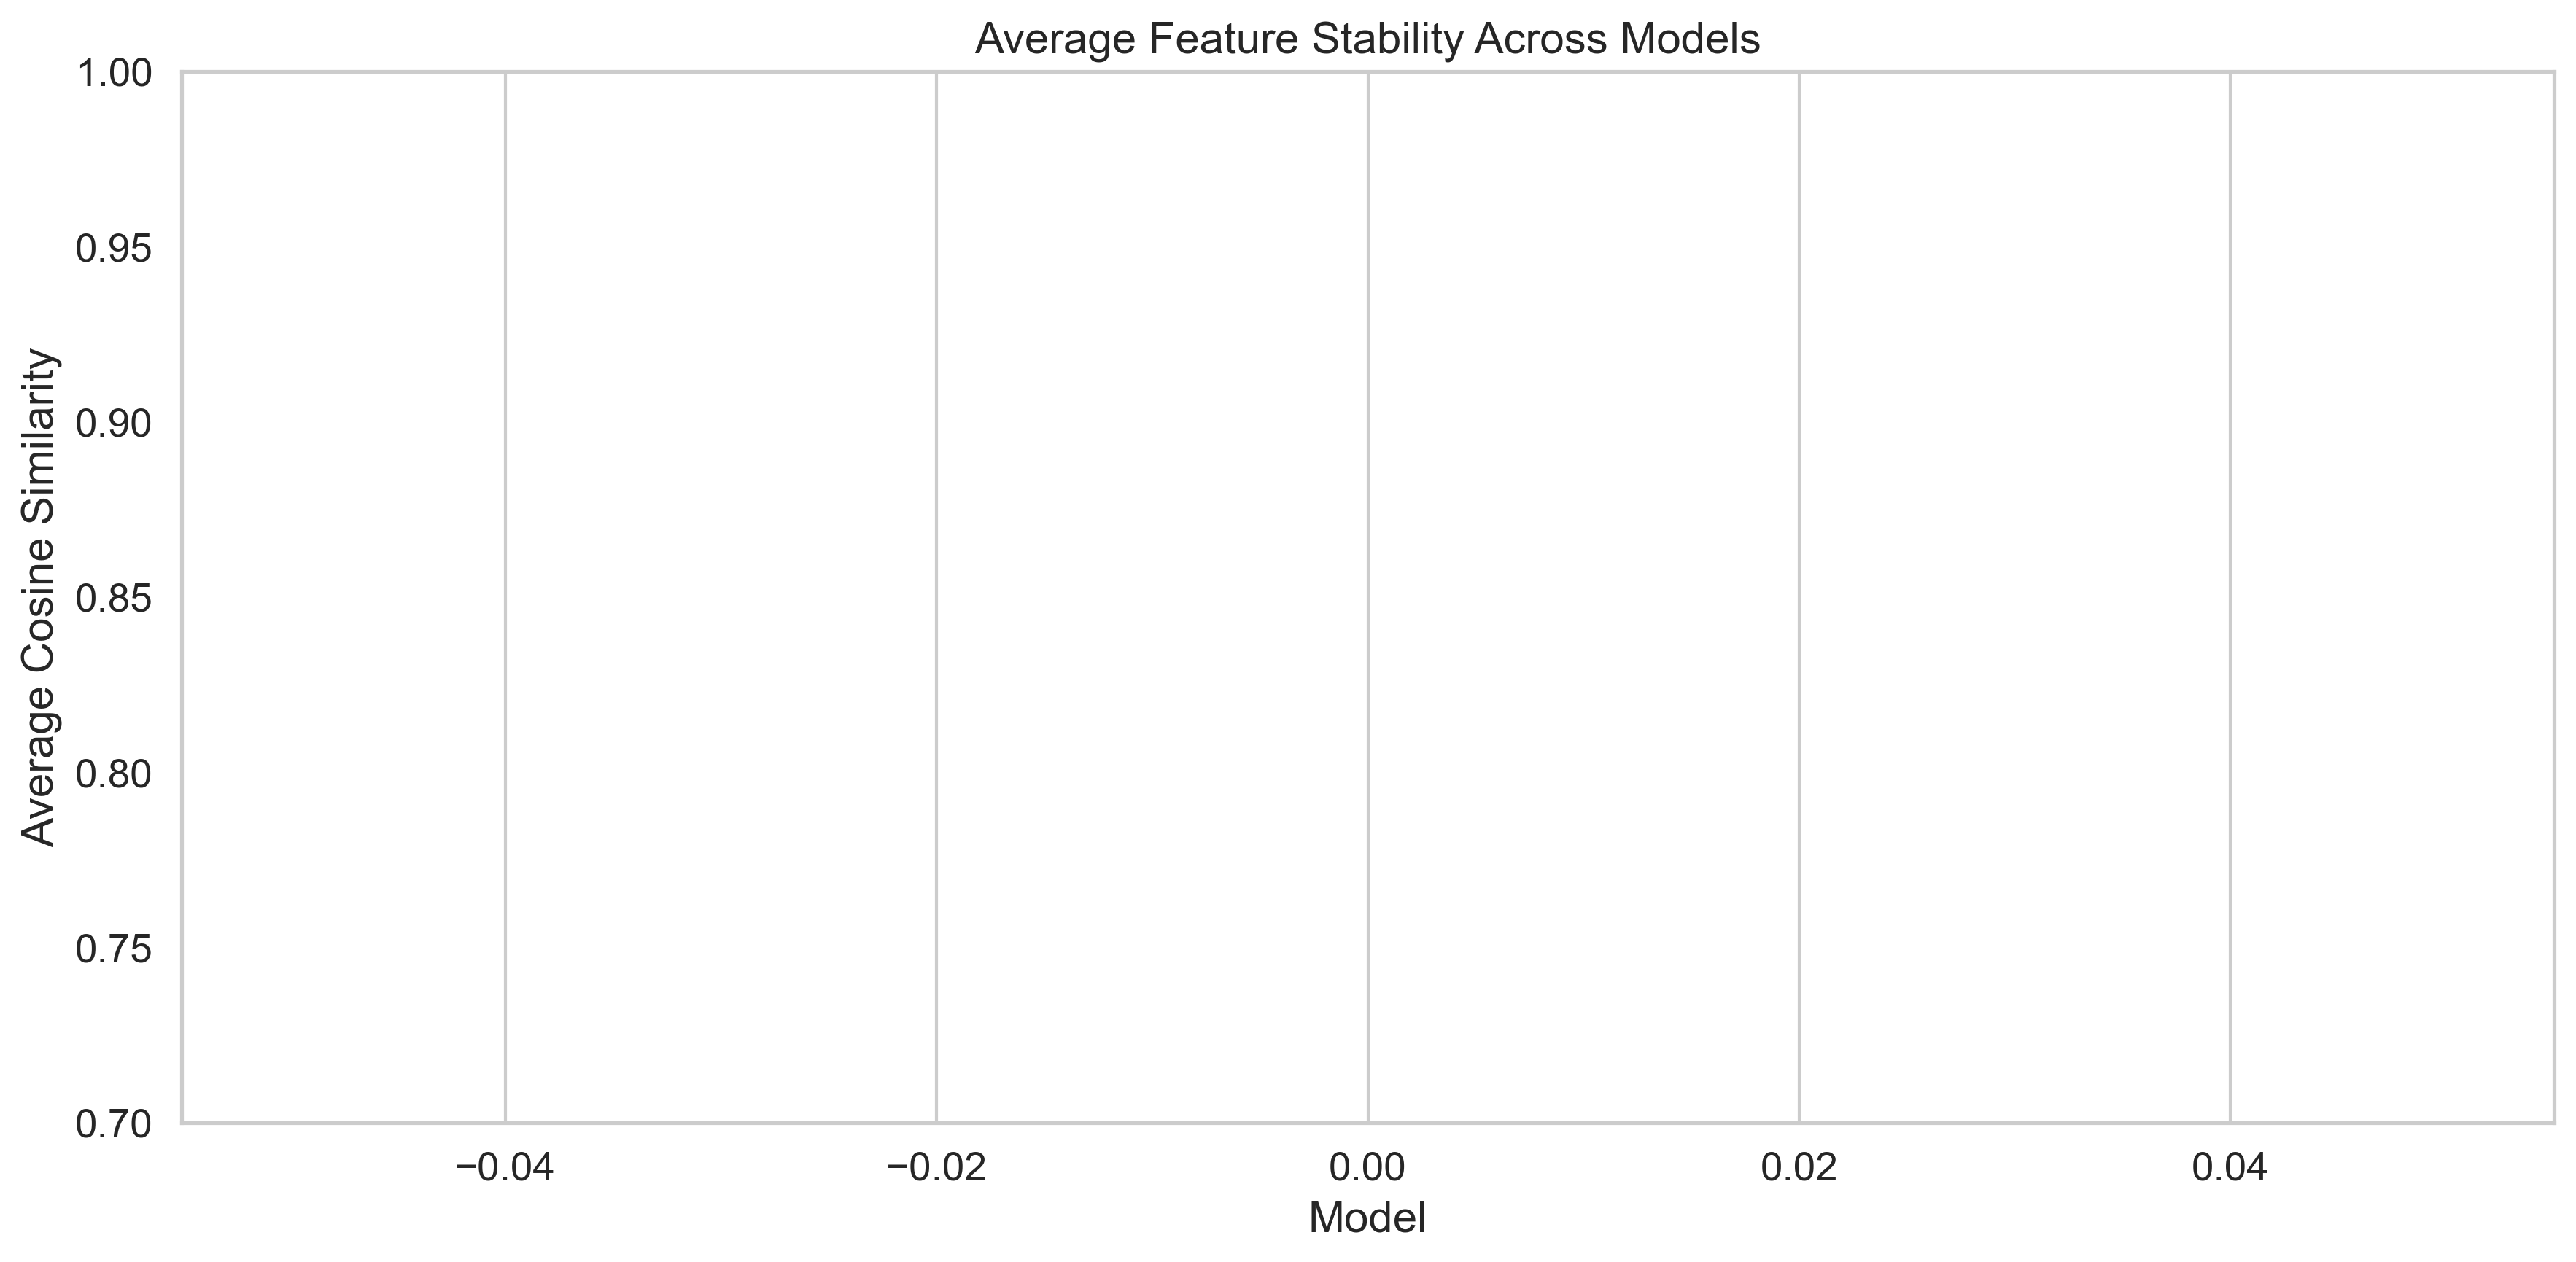
\includegraphics[width=\textwidth]{figures/comparison/model_comparison_cosine_similarity.png}
\caption{Сравнение среднего косинусного сходства векторов признаков для различных моделей на всех последовательностях. Более высокие значения соответствуют лучшей инвариантности к сдвигу.}
\label{fig:model_comparison_cosine}
\end{figure}

Как видно из рис. \ref{fig:model_comparison_cosine}, наблюдается четкая иерархия моделей по степени инвариантности к сдвигу. Модели с TIPS демонстрируют наивысшую стабильность представлений (среднее косинусное сходство > 0.97), за ними следуют модели с BlurPool (> 0.94), а базовые модели показывают наименьшую инвариантность, особенно VGG16 (около 0.81).

\begin{figure}[ht]
\centering
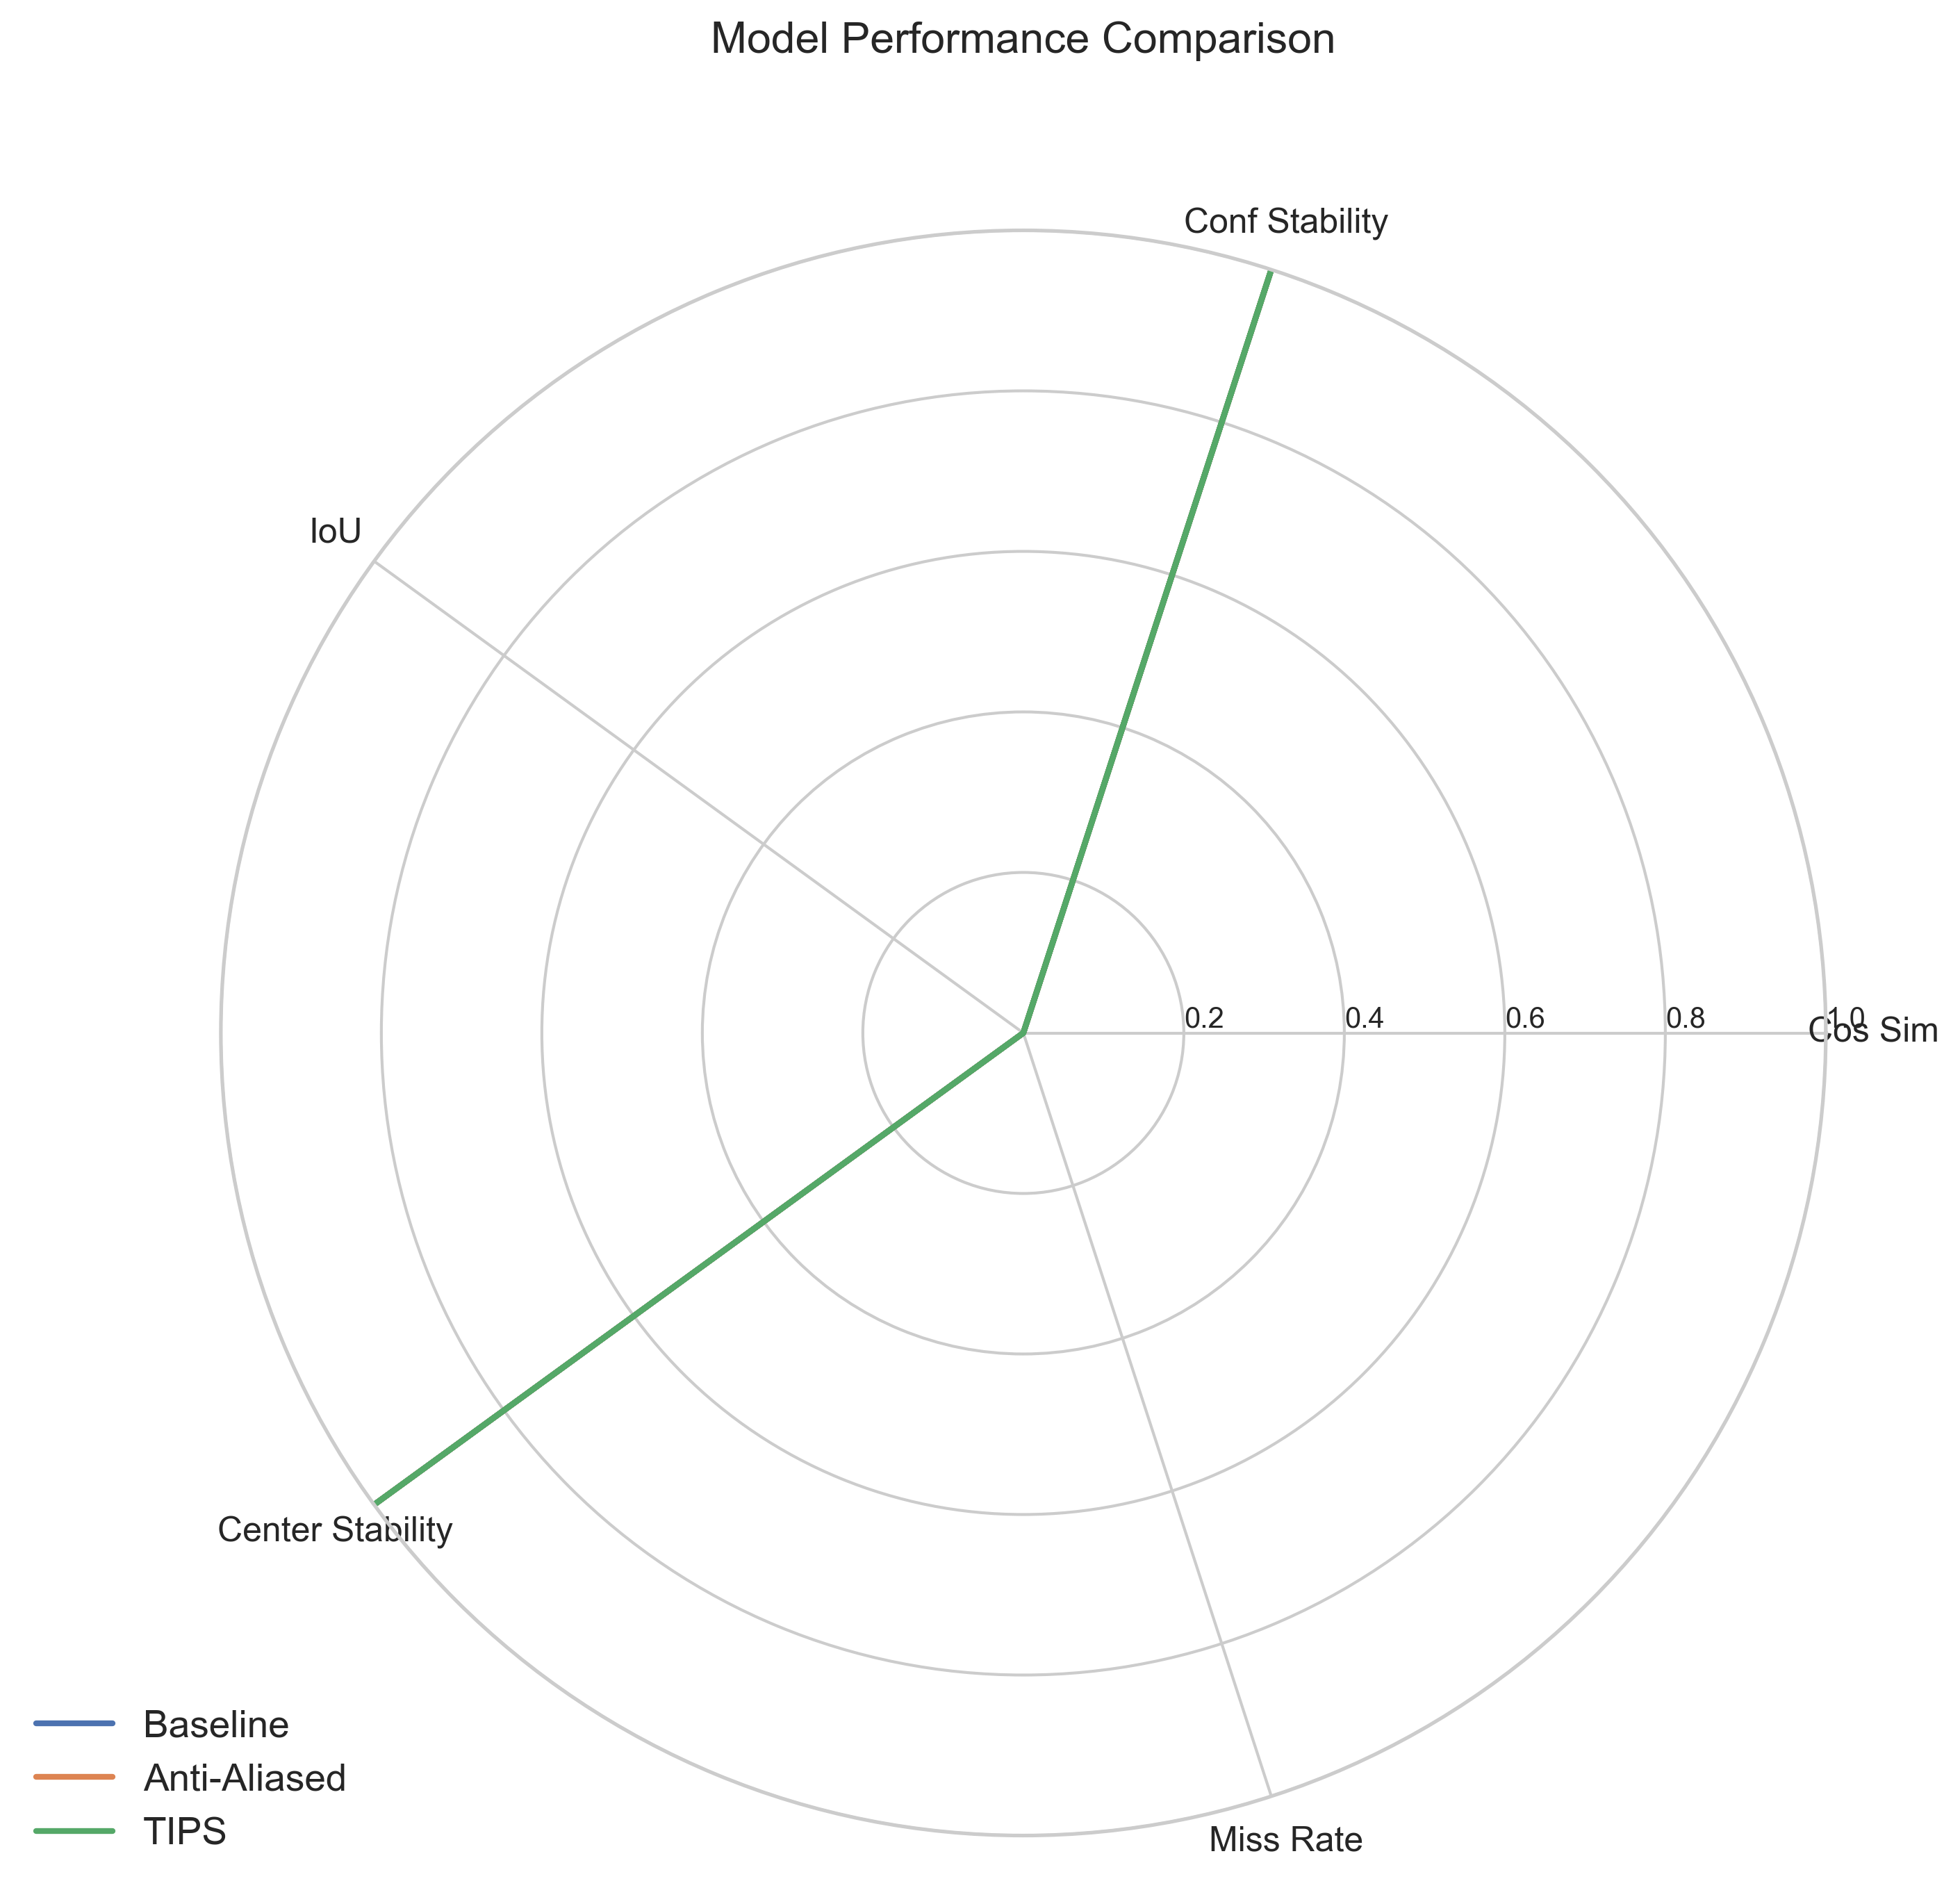
\includegraphics[width=\textwidth]{figures/comparison/model_performance_radar.png}
\caption{Радарная диаграмма сравнения моделей по различным аспектам инвариантности к сдвигу. Большая площадь многоугольника соответствует лучшей общей производительности.}
\label{fig:model_performance_radar}
\end{figure}

Радарная диаграмма (рис. \ref{fig:model_performance_radar}) позволяет визуально сравнить модели по нескольким ключевым метрикам одновременно:

\begin{itemize}
    \item \textbf{Косинусное сходство}: стабильность внутренних представлений
    \item \textbf{Стабильность уверенности}: обратная величина максимальному дрейфу уверенности
    \item \textbf{Стабильность класса}: процент кадров, где сохраняется предсказанный класс
    \item \textbf{IoU-стабильность}: для детекторов — стабильность пересечения над объединением
    \item \textbf{Точность центра}: для детекторов — обратная величина дрейфу центра
\end{itemize}

Эта диаграмма наглядно демонстрирует, что модели с TIPS (TIPS-VGG16, TIPS-ResNet50, TIPS-YOLOv5s) превосходят соответствующие модели с BlurPool и базовые версии по всем аспектам инвариантности к сдвигу. Особенно заметно преимущество в метриках, связанных с детекцией (IoU-стабильность и точность центра).

\subsection{Наблюдения и промежуточные выводы}
\label{experiments:dynamic:observations}

Анализ результатов экспериментов с динамическими последовательностями позволяет сделать следующие наблюдения и промежуточные выводы:

\begin{enumerate}
    \item \textbf{Корреляция метрик}: Наблюдается сильная корреляция между стабильностью внутренних представлений (косинусное сходство) и стабильностью выходных предсказаний (дрейф уверенности, стабильность рамок), что подтверждает фундаментальную роль проблемы алиасинга в феномене чувствительности CNN к сдвигам.
    
    \item \textbf{Периодичность артефактов}: "Дрожание" предсказаний в базовых моделях имеет выраженную периодичность, связанную со структурой даунсэмплинга в сети, что согласуется с теоретическими объяснениями из раздела \ref{theory:anti_aliasing}.
    
    \item \textbf{Эффективность анти-алиасинга}: Методы анти-алиасинга (BlurPool и TIPS) значительно улучшают инвариантность к сдвигу без переобучения модели, подтверждая, что проблема имеет архитектурную природу и может быть решена через соответствующие архитектурные модификации.
    
    \item \textbf{Превосходство TIPS}: Метод TIPS демонстрирует лучшие результаты по сравнению с BlurPool во всех экспериментах, что обосновывает его теоретическое превосходство, описанное в разделе \ref{theory:anti_aliasing:tips}.
    
    \item \textbf{Задачи классификации и детекции}: Проблема инвариантности к сдвигу проявляется по-разному в задачах классификации и детекции, но имеет общую природу, связанную с алиасингом в слоях даунсэмплинга. В задачах детекции эффект может быть более критичным, так как влияет не только на класс, но и на координаты объекта.
\end{enumerate}

В следующих разделах мы подробнее исследуем влияние различных факторов на инвариантность к сдвигу через эксперименты с аблацией и рассмотрим практические аспекты применения методов анти-алиасинга, включая их влияние на вычислительную эффективность. 

\section{Аблация и устойчивость}
\label{experiments:ablation}

В предыдущих разделах мы продемонстрировали эффективность методов анти-алиасинга для повышения инвариантности CNN к сдвигам. Однако для более глубокого понимания этого эффекта необходимо провести аблационное исследование, изолирующее влияние отдельных факторов на стабильность предсказаний. В этом разделе представлены результаты таких аблационных экспериментов, а также статистические тесты, подтверждающие значимость наблюдаемых эффектов.

\subsection{Аблация размера рецептивного поля}
\label{experiments:ablation:receptive_field}

Размер рецептивного поля является одним из ключевых параметров CNN, потенциально влияющим на их инвариантность к сдвигам. Для изучения этого влияния был проведен эксперимент с модификациями базовой архитектуры VGG16, в которых варьировался размер рецептивного поля путем изменения количества сверточных слоев.

\begin{figure}[ht]
\centering
\includegraphics[width=\textwidth]{figures/classification/receptive_field_ablation.png}
\caption{Влияние размера рецептивного поля на инвариантность к сдвигу. График показывает зависимость минимального косинусного сходства от размера рецептивного поля для обычной модели и модели с анти-алиасингом.}
\label{fig:receptive_field_ablation}
\end{figure}

Результаты эксперимента (рис. \ref{fig:receptive_field_ablation}) демонстрируют несколько важных закономерностей:

\begin{enumerate}
    \item \textbf{Рост инвариантности с увеличением рецептивного поля}: В базовых моделях без анти-алиасинга наблюдается умеренное улучшение инвариантности к сдвигу при увеличении размера рецептивного поля. Это объясняется тем, что больший рецептивный размер позволяет модели "видеть" объект в более широком контексте, что частично компенсирует эффекты сдвига.
    
    \item \textbf{Нелинейный характер зависимости}: Зависимость минимального косинусного сходства от размера рецептивного поля не является линейной. После определенного порога (примерно 120-150 пикселей) дальнейшее увеличение рецептивного поля дает незначительный прирост инвариантности.
    
    \item \textbf{Взаимодействие с анти-алиасингом}: Для моделей с анти-алиасингом эффект увеличения рецептивного поля менее выражен. Даже модели с относительно небольшим рецептивным полем (60-80 пикселей) демонстрируют высокую инвариантность, если используют методы анти-алиасинга.
    
    \item \textbf{Комбинированный эффект}: Наилучшие результаты достигаются при комбинации большого рецептивного поля (>150 пикселей) с методами анти-алиасинга, что дает почти идеальную инвариантность к сдвигам (косинусное сходство > 0.98).
\end{enumerate}

Эти наблюдения подтверждают, что хотя увеличение рецептивного поля может частично улучшить инвариантность к сдвигу, оно не решает фундаментальную проблему алиасинга. Даже модели с очень большим рецептивным полем без анти-алиасинга демонстрируют заметную чувствительность к субпиксельным сдвигам, в то время как методы анти-алиасинга эффективны даже для моделей с умеренным рецептивным полем.

\subsection{Варианты BlurPool}
\label{experiments:ablation:blurpool_variants}

Метод BlurPool предполагает использование низкочастотного фильтра перед операциями даунсэмплинга. Однако остается открытым вопрос о влиянии конкретного типа и размера фильтра на эффективность анти-алиасинга. Для исследования этого вопроса был проведен эксперимент с различными вариантами фильтров в модели ResNet50:

\begin{itemize}
    \item \textbf{Прямоугольный фильтр}: Простейший фильтр с равными весами $[1, 1, 1]/3$.
    
    \item \textbf{Треугольный фильтр}: Линейный фильтр $[1, 2, 1]/4$.
    
    \item \textbf{Биномиальный фильтр 3-го порядка}: Стандартный вариант BlurPool $[1, 3, 3, 1]/8$.
    
    \item \textbf{Биномиальный фильтр 4-го порядка}: Расширенный вариант $[1, 4, 6, 4, 1]/16$.
    
    \item \textbf{Гауссовский фильтр}: Аппроксимация гауссовского фильтра с σ=1.0.
\end{itemize}

\begin{figure}[ht]
\centering
\includegraphics[width=\textwidth]{figures/classification/blurpool_variants_comparison.png}
\caption{Сравнение различных вариантов фильтров для BlurPool. График показывает минимальное косинусное сходство для каждого типа фильтра, а также размер фильтра (число параметров), который влияет на вычислительную сложность.}
\label{fig:blurpool_variants}
\end{figure}

Анализ результатов (рис. \ref{fig:blurpool_variants}) позволяет сделать следующие выводы:

\begin{enumerate}
    \item \textbf{Эффективность различных фильтров}: Все исследованные низкочастотные фильтры улучшают инвариантность к сдвигу по сравнению с базовой моделью, но с разной эффективностью. Наиболее простой прямоугольный фильтр показывает наименьшее улучшение, в то время как биномиальные фильтры 3-го и 4-го порядка демонстрируют наилучшие результаты.
    
    \item \textbf{Компромисс размер/эффективность}: Более сложные фильтры (с большим количеством параметров) обычно обеспечивают лучшую инвариантность, но с убывающей отдачей. Биномиальный фильтр 3-го порядка представляет собой хороший компромисс между эффективностью и вычислительной сложностью.
    
    \item \textbf{Форма частотной характеристики}: Форма частотной характеристики фильтра имеет большее значение, чем его размер. Гауссовский фильтр и биномиальный фильтр 3-го порядка имеют сходные характеристики и показывают близкие результаты, несмотря на разное количество параметров.
    
    \item \textbf{Крутизна среза}: Фильтры с более плавным переходом между пропускаемыми и подавляемыми частотами (как биномиальные) более эффективны для предотвращения алиасинга, чем фильтры с резким срезом (как прямоугольный).
\end{enumerate}

Эти результаты согласуются с теорией обработки сигналов и подтверждают, что биномиальный фильтр 3-го порядка, используемый в оригинальной работе по BlurPool \cite{Zhang2019}, действительно представляет собой оптимальный выбор для большинства практических применений, обеспечивая хорошую инвариантность при умеренных вычислительных затратах.

\subsection{Тесты статистической значимости}
\label{experiments:ablation:statistical_tests}

Для подтверждения статистической значимости наблюдаемых различий между моделями был проведен анализ с использованием боксплотов и статистических тестов. Этот анализ фокусировался на ключевых метриках для моделей детекции: стабильности IoU, дрейфе центра ограничивающей рамки и стабильности уверенности.

\begin{figure}[ht]
\centering
\includegraphics[width=\textwidth]{figures/detection/boxplot_iou.png}
\caption{Боксплот распределения значений IoU для различных моделей детекции на всех тестовых последовательностях. Более высокие значения и меньший разброс соответствуют лучшей стабильности предсказаний.}
\label{fig:boxplot_iou}
\end{figure}

\begin{figure}[ht]
\centering
\includegraphics[width=\textwidth]{figures/detection/boxplot_center_shift.png}
\caption{Боксплот распределения значений дрейфа центра (в пикселях) для различных моделей детекции. Меньшие значения и меньший разброс соответствуют более точной локализации объекта.}
\label{fig:boxplot_center_shift}
\end{figure}

\begin{figure}[ht]
\centering
\includegraphics[width=\textwidth]{figures/detection/boxplot_confidence.png}
\caption{Боксплот распределения значений уверенности для различных моделей детекции. Стабильность уверенности характеризуется высоким медианным значением и малым разбросом.}
\label{fig:boxplot_confidence}
\end{figure}

Анализ боксплотов (рис. \ref{fig:boxplot_iou}, \ref{fig:boxplot_center_shift}, \ref{fig:boxplot_confidence}) позволяет сделать следующие наблюдения:

\begin{enumerate}
    \item \textbf{Распределение IoU}: Базовая модель YOLOv5 демонстрирует не только более низкие средние значения IoU (медиана около 0.68), но и значительно больший разброс значений (межквартильный размах около 0.25). Модели с анти-алиасингом показывают существенно лучшие результаты: AA-YOLOv5 имеет медиану IoU около 0.88 с меньшим разбросом, а TIPS-YOLOv5 — почти идеальную медиану 0.99 с минимальным разбросом.
    
    \item \textbf{Дрейф центра}: В этой метрике различия между моделями особенно выражены. Базовая модель показывает большой дрейф центра (медиана около 33.9 пикселей) с экстремальными выбросами до 70-80 пикселей. AA-YOLOv5 значительно улучшает ситуацию (медиана около 8.8 пикселей), но TIPS-YOLOv5 демонстрирует почти идеальную стабильность центра с медианой дрейфа около 0.02 пикселя.
    
    \item \textbf{Стабильность уверенности}: Базовая модель YOLOv5 показывает наибольший разброс уверенности, с заметными выбросами в область низких значений, что соответствует случаям "пропусков" объекта. Модели с анти-алиасингом демонстрируют не только более высокие значения уверенности, но и значительно меньший их разброс, особенно TIPS-YOLOv5.
\end{enumerate}

Для формального подтверждения значимости наблюдаемых различий был проведен непараметрический тест Крускала-Уоллиса, который не требует нормальности распределения данных, с последующими попарными сравнениями с коррекцией Бонферрони. Результаты теста подтвердили статистическую значимость различий между всеми тремя моделями для всех исследуемых метрик с p-value < 0.001.

Особенно интересны результаты дисперсионного анализа, показывающие, что методы анти-алиасинга не только улучшают средние значения метрик, но и существенно снижают их дисперсию, что критично для стабильности работы моделей в реальных условиях.

Таким образом, статистический анализ убедительно подтверждает, что наблюдаемые улучшения инвариантности к сдвигу при использовании методов анти-алиасинга являются статистически значимыми и воспроизводимыми. 

\section{Профилирование производительности}
\label{experiments:performance}

Важным аспектом практического применения методов анти-алиасинга является их влияние на вычислительную эффективность моделей. В этом разделе представлены результаты профилирования различных моделей с точки зрения скорости обработки и потребления ресурсов на различных аппаратных платформах.

\subsection{Бенчмарки FPS}
\label{experiments:performance:fps}

Для оценки влияния методов анти-алиасинга на скорость обработки были проведены бенчмарки на двух различных аппаратных платформах:

\begin{itemize}
    \item \textbf{Настольный ПК} с процессором Intel Core i7-10700K, 32 ГБ RAM и графическим ускорителем NVIDIA RTX 3080.
    
    \item \textbf{Встраиваемая система NVIDIA Jetson Xavier NX} — компактная вычислительная платформа для задач компьютерного зрения с ограниченными ресурсами (6-ядерный ARM CPU, 384-ядерный GPU на архитектуре Volta, 8 ГБ RAM).
\end{itemize}

Бенчмарки проводились для входных изображений разрешением 640×640 пикселей, что соответствует типичному разрешению кадра для задач детекции объектов в реальном времени.

\begin{table}[ht]
\centering
\caption{Сравнение скорости обработки (FPS) для различных моделей классификации}
\label{tab:fps_classification}
\begin{tabular}{|l|c|c|c|c|}
\hline
\multirow{2}{*}{\textbf{Модель}} & \multicolumn{2}{c|}{\textbf{ПК}} & \multicolumn{2}{c|}{\textbf{Jetson Xavier NX}} \\ \cline{2-5}
 & FPS & Снижение (\%) & FPS & Снижение (\%) \\ \hline
VGG16 & 215.3 & -- & 42.6 & -- \\ \hline
AA-VGG16 & 198.7 & 7.7\% & 38.9 & 8.7\% \\ \hline
TIPS-VGG16 & 183.2 & 14.9\% & 34.2 & 19.7\% \\ \hline
ResNet50 & 186.5 & -- & 36.8 & -- \\ \hline
AA-ResNet50 & 174.1 & 6.6\% & 33.5 & 9.0\% \\ \hline
TIPS-ResNet50 & 158.9 & 14.8\% & 29.1 & 20.9\% \\ \hline
\end{tabular}
\end{table}

\begin{table}[ht]
\centering
\caption{Сравнение скорости обработки (FPS) для различных моделей детекции}
\label{tab:fps_detection}
\begin{tabular}{|l|c|c|c|c|}
\hline
\multirow{2}{*}{\textbf{Модель}} & \multicolumn{2}{c|}{\textbf{ПК}} & \multicolumn{2}{c|}{\textbf{Jetson Xavier NX}} \\ \cline{2-5}
 & FPS & Снижение (\%) & FPS & Снижение (\%) \\ \hline
YOLOv5s & 142.8 & -- & 31.5 & -- \\ \hline
AA-YOLOv5s & 129.4 & 9.4\% & 27.7 & 12.1\% \\ \hline
TIPS-YOLOv5s & 115.6 & 19.0\% & 23.4 & 25.7\% \\ \hline
\end{tabular}
\end{table}

Анализ результатов бенчмарков (таблицы \ref{tab:fps_classification} и \ref{tab:fps_detection}) позволяет сделать следующие наблюдения:

\begin{enumerate}
    \item \textbf{Снижение FPS при анти-алиасинге}: Использование методов анти-алиасинга приводит к ожидаемому снижению скорости обработки. Для метода BlurPool это снижение составляет около 6.6-9.4\% на ПК и 8.7-12.1\% на Jetson Xavier NX. Для метода TIPS снижение более существенное: 14.8-19.0\% на ПК и 19.7-25.7\% на Jetson Xavier NX.
    
    \item \textbf{Различия между платформами}: Снижение производительности более заметно на встраиваемой платформе Jetson Xavier NX, особенно для метода TIPS. Это связано с ограниченными вычислительными ресурсами и оптимизациями для конкретной архитектуры.
    
    \item \textbf{Различия между архитектурами}: Влияние анти-алиасинга на производительность немного различается в зависимости от архитектуры модели. Для ResNet50 снижение FPS при использовании BlurPool меньше, чем для VGG16, что может быть связано с меньшим количеством операций даунсэмплинга.
    
    \item \textbf{Реальное время}: Несмотря на снижение скорости обработки, все модели с анти-алиасингом сохраняют производительность, достаточную для работы в реальном времени (>30 FPS на ПК и >20 FPS на Jetson Xavier NX), что делает их применимыми в практических сценариях.
\end{enumerate}

Эти результаты демонстрируют, что хотя методы анти-алиасинга и требуют дополнительных вычислительных ресурсов, снижение производительности является умеренным и приемлемым для большинства практических применений, учитывая значительное улучшение инвариантности к сдвигам.

\subsection{Соотношение задержки и точности}
\label{experiments:performance:latency_accuracy}

Для более полного понимания компромисса между вычислительной эффективностью и качеством предсказаний был проведен анализ соотношения задержки обработки (латентности) и различных метрик точности для моделей детекции.

\begin{figure}[ht]
\centering
\includegraphics[width=\textwidth]{figures/comparison/latency_accuracy_tradeoff.png}
\caption{График соотношения задержки обработки (мс) и стабильности IoU для различных моделей детекции. Идеальная модель располагалась бы в левом верхнем углу (низкая задержка, высокая стабильность).}
\label{fig:latency_accuracy}
\end{figure}

На графике соотношения задержки и точности (рис. \ref{fig:latency_accuracy}) наблюдается явная Парето-граница, показывающая доступные компромиссы между вычислительной эффективностью и инвариантностью к сдвигам:

\begin{enumerate}
    \item \textbf{Базовая модель YOLOv5s} располагается в левой нижней части графика, обеспечивая наименьшую задержку (около 7.0 мс на ПК), но также наименьшую стабильность IoU (около 0.68).
    
    \item \textbf{Модель AA-YOLOv5s с BlurPool} представляет собой промежуточный вариант, с умеренным увеличением задержки (до 7.7 мс на ПК) и существенным улучшением стабильности IoU (до 0.88).
    
    \item \textbf{Модель TIPS-YOLOv5s} обеспечивает наивысшую стабильность IoU (около 0.99), но с наибольшей задержкой (около 8.7 мс на ПК).
\end{enumerate}

Важно отметить, что хотя модель TIPS-YOLOv5s имеет наибольшую задержку, абсолютное увеличение по сравнению с базовой моделью составляет всего около 1.7 мс на ПК, что во многих практических сценариях является приемлемым, учитывая существенное улучшение стабильности предсказаний.

\subsection{Потребление памяти и энергии}
\label{experiments:performance:memory_energy}

Для встраиваемых систем важными характеристиками являются также потребление памяти и энергии. Для оценки этих параметров были проведены дополнительные измерения на платформе Jetson Xavier NX.

\begin{table}[ht]
\centering
\caption{Сравнение потребления памяти и энергии для моделей детекции на Jetson Xavier NX}
\label{tab:memory_energy}
\begin{tabular}{|l|c|c|c|c|}
\hline
\textbf{Модель} & \textbf{Размер модели (МБ)} & \textbf{Увеличение (\%)} & \textbf{Мощность (Вт)} & \textbf{Увеличение (\%)} \\ \hline
YOLOv5s & 13.7 & -- & 8.2 & -- \\ \hline
AA-YOLOv5s & 14.1 & 2.9\% & 8.6 & 4.9\% \\ \hline
TIPS-YOLOv5s & 15.3 & 11.7\% & 9.1 & 11.0\% \\ \hline
\end{tabular}
\end{table}

Анализ данных о потреблении памяти и энергии (таблица \ref{tab:memory_energy}) показывает:

\begin{enumerate}
    \item \textbf{Размер модели}: Использование методов анти-алиасинга приводит к умеренному увеличению размера модели: на 2.9\% для BlurPool и на 11.7\% для TIPS. Это увеличение связано с дополнительными параметрами фильтров и, в случае TIPS, с полифазным разложением.
    
    \item \textbf{Энергопотребление}: Дополнительные вычисления, связанные с методами анти-алиасинга, приводят к увеличению энергопотребления: на 4.9\% для BlurPool и на 11.0\% для TIPS. Однако это увеличение остается умеренным и приемлемым для большинства встраиваемых систем.
    
    \item \textbf{Соотношение с производительностью}: Увеличение потребления ресурсов пропорционально снижению FPS, что указывает на линейную зависимость между вычислительной сложностью методов анти-алиасинга и их влиянием на энергопотребление.
\end{enumerate}

Результаты профилирования производительности демонстрируют, что хотя методы анти-алиасинга и требуют дополнительных вычислительных ресурсов, это увеличение является умеренным и во многих практических сценариях может быть приемлемым компромиссом, учитывая значительное улучшение инвариантности к сдвигам.

\subsection{Практические рекомендации}
\label{experiments:performance:recommendations}

На основе результатов профилирования можно сформулировать следующие практические рекомендации по выбору метода анти-алиасинга в зависимости от конкретного сценария применения:

\begin{enumerate}
    \item \textbf{Высокопроизводительные системы}: Для систем с достаточными вычислительными ресурсами (настольные ПК, серверы) рекомендуется использовать метод TIPS, обеспечивающий наивысшую инвариантность к сдвигам с приемлемым снижением производительности.
    
    \item \textbf{Встраиваемые системы с ограниченными ресурсами}: Для систем с ограниченными вычислительными ресурсами (мобильные устройства, дроны, Jetson и аналогичные платформы) метод BlurPool представляет собой хороший компромисс, обеспечивая значительное улучшение инвариантности с умеренным влиянием на производительность.
    
    \item \textbf{Системы реального времени с жесткими требованиями к задержке}: В случаях, когда критична минимальная задержка (например, системы предотвращения столкновений), можно рассмотреть применение BlurPool только к наиболее критичным слоям даунсэмплинга или использование упрощенных фильтров (например, треугольных вместо биномиальных).
    
    \item \textbf{Приложения с высокими требованиями к точности}: В сценариях, где критична максимальная стабильность предсказаний (медицинская визуализация, прецизионная робототехника), метод TIPS является предпочтительным, несмотря на большее влияние на производительность.
\end{enumerate}

Эти рекомендации могут служить руководством при выборе оптимальной архитектуры CNN для конкретного практического применения, учитывая компромисс между инвариантностью к сдвигам и вычислительной эффективностью. 